
\section{Resultados}

\subsection{Red de interacciones y robustez}

La siguiente imagen muestra la red de interaciones del ser humano con las proteínas del SARS-CoV. Como podemos ver el SARS-CoV interacciona con 89 proteínas humanas, produciendo un total de 475 interacciones. 
\begin{center}
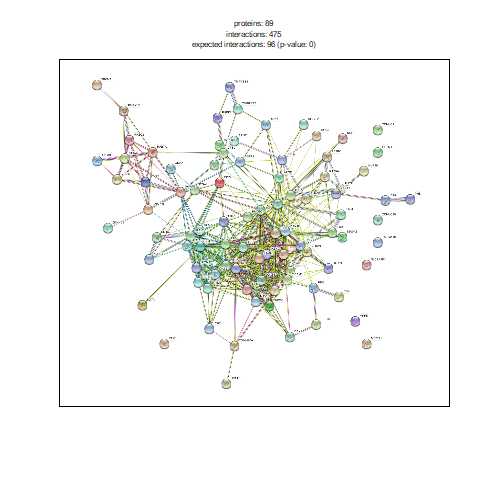
\includegraphics[width=70mm,scale=1.2]{report/figures/string_hits.png}
\caption{\textit{Red de interacciones del SARS-CoV con las proteínas humanas }}
\end{center}

Tras eliminar los nodos que no están conectados, hemos obtenido la red real de interacciones que podemos ver a continuación. Sin embargohay demasiadas conexiones como para poder distinguir los nodos. Es por ello que realizaremos los pasos siguientes de clustering, para así poder extraer la informaión relevante de la red. 
\begin{center}
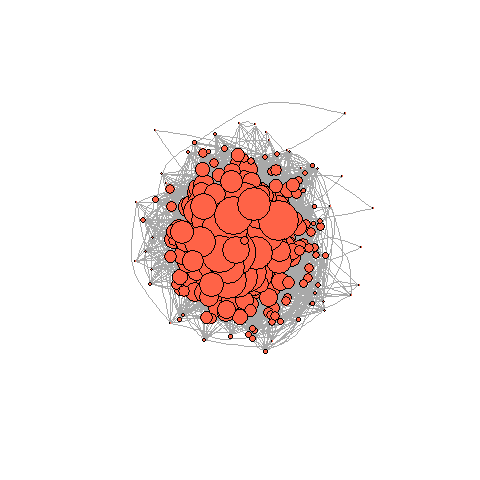
\includegraphics[width=70mm,scale=1.2]{report/figures/hits.network_graph.png}
\caption{\textit{Red de interacciones del SARS-CoV con las proteínas humanas tras un proceso de filtrado}}
\end{center}

Para poder estudiar cual es la capacidad de nuestra red de mantener sus funciones frente a la presencia de "ataques" y ver cuán de adaptable es, usamos la robustez. Podemos observar que para ataques aleatorios es bastante robusta, mientras que para ataques dirigidos es más débil. 
\begin{center}
	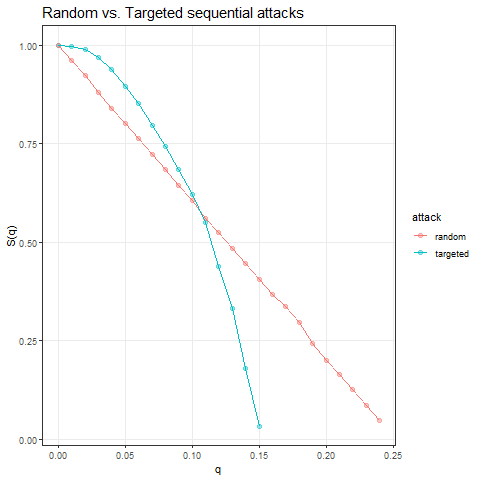
\includegraphics[width=70mm,scale=1.2]{report/figures/sequential_attacks.png}
	\caption{\textit{Robustez frente a ataques dirigidos y aleatorios}}
\end{center}

\subsection{Clustering}




